\documentclass[stage]{tnreport}

\usepackage[utf8]{inputenc} 

\def\reportTitle{Mise en place d’un service de compilation/d’exécution isolé pour la plateforme PLM dédiée à l’apprentissage de la programmation} % Titre du mémoire
\def\reportLongTitle{Mise en place d’un service de compilation/d’exécution isolé pour la plateforme PLM dédiée à l’apprentissage de la programmation} % Titre plus long du mémoire

\def\reportAuthor{Tanguy GLOAGUEN}
\def\reportAuthorEmail{\email{tanguy.gloaguen@telecomnancy.eu}} % Courriel de l'élève

\def\reportSupervisor{Martin QUINSON, Gérald OSTER} % Prénom Nom de l'encadrant industriel

\def\reportCompany{LORIA} % Nom de l'entreprise d'accueil
\def\reportCompanyAddress{Campus Scientifique}  % Adresse de l'entreprise
\def\reportCompanyCity{54506, Nancy} % Adresse (cont.) de l'entreprise
\def\reportCompanyPhone{~} % Téléphone de l'entreprise
\def\reportCompanyLogoPath{figures/LORIA-logo.jpg} % Logo de l'entreprise

\def\place{Nancy} % Ville pour la signature pour l'engagement anti-plagiat
\def\date{\today} % Date pour la signature de l'engagement anti-plagiat

\def\reportProjectCustomer{}

\begin{document}

\maketitle
\pagenumbering{roman}

\insertAntiPlagiarismAgreement{GLOAGUEN, Tanguy}{31313847}

\cleardoublepage

\makesecondtitle

\section*{Remerciements}
\addcontentsline{toc}{chapter}{Remerciements}

{\em
Je tiens tout d'abord à remercier mes encadrants de stage, MM. Oster et Quinson, pour leur accueil au sein de leur équipe, leurs conseils et explications sur le système à étudier et le temps qu'ils ont accordé à l'étude des modèles proposés.

Je remercie également Matthieu Nicolas, qui m'a également encadré lors de ce stage, pour son aide précieuse sur les outils à utiliser, mais aussi pour son écoute et ses conseils quant aux méthodes de résolution des problèmes étudiés.

Enfin, je remercie mes collègues de bureau, MM. Bühler, Carpentier et Grguric, pour leurs aides sur la réqlisation et pour l'ambiance agréable de travail.
}

\cleardoublepage

\renewcommand{\baselinestretch}{0.5}\normalsize
\tableofcontents
\renewcommand{\baselinestretch}{1.0}\normalsize
\cleardoublepage

\pagenumbering{arabic}
\setcounter{page}{1}

\chapter*{Introduction}

L'enseignement classique est celui généralement utilisé aujourd'hui, mais l'accés au public de l'informatique a permi de mettre en place des apprentissages plus automatisés : outils d'aide à l'enseignement, MOOC (cours en ligne) mais aussi logiciels d'apprentissage autonome.
C'est dans ce contexte que se place la Programmer's Learning Machine : depuis 2007, cette application permet de standardiser les enseignements de base en programmation ainsi que d'aider les enseignants à évaluer les progrès des élèves.
La PLM a pour but d'enseigner les bases de la programmation et de fournir aux éudiants les meilleurs outils possibles pour apprendre à coder.

En vue de moderniser le logiciel, il a été récemment proposé de transformer l'application PLM en un outil en ligne. Cette modification a entraîné des contraintes de sécurité, de puissance du matériel, de consommation mémoire et processeur des services et de mise à l'échelle supplémentaires qu'il a fallu résoudre.

L'objectif de ce stage était de proposer des solutions à ces contraintes, de les implémenter et de proposer des méthodes de déploiement.

Dans un premier temps, nous verrons le contexte du stage plus en détail : l'établissement d'accueil mais aussi la Programmer's Learning Machine en tant qu'application et qu'interface web.

Dans un second temps, nous verrons les objectifs du stage.

Puis, nous étudierons la réalisation de ces objectifs en tant que méthodologie, en tant qu'environnement et les résultats obtenus.

Enfin, nous ferons un bilan des résultats et une liste des améliorations prévues et possibles.

\cleardoublepage

\chapter{Présentation}

\section{le LORIA}

Le Laboratoire Lorrain de Recherche en Informatique et ses Applications (abrégé LORIA) est une Unité Mixe de Recherche créé en 1997 par association entre le CNRS (Centre National de la Recherche Scientifique), l'UL (Université de Lorraine) et l'INRIA (Institut National de Recherche en Informatique et Automatique).

La mission principale du LORIA est la recherche fondamentale et appliquée dans le cadre des sciences informatiques. Elle accueille un total de 450 personnes\footnote{chiffres 2014, http://www.loria.fr/rapports-activite-2/rapport-dactivite-2014}, réparties en 27 équipes sur 5 dépatements :
\begin{description}
	\item[Algorithmique, calcul, image et géométrie] \hfill \\
		Ce département de 6 équipes, dirigé par Sylvain Lazard, s'intéresse principalement aux algorithmes tout en gardant une différence sur les applications selon les équipes.
	\item[Méthodes formelles] \hfill \\
		 Ce département de 6 équipes, dirigé par Dominique Méry, développe des contributions aux logiques et théories de preuves. C'est dans ce département que se trouve VERIDIS et le projet PLM.
	\item[Réseaux, systèmes et services] \hfill \\
		 Département de 3 équipes dirigé par Ye-Quiong Song, il s'intéresse principalement aux problèmes issus des systèmes distribués et parallèles.
	\item[Traitement des langues et des connaissances] \hfill \\
		 Ce département de 8 équipes dirigé par Bruno Guillaume porte sur l'étude des langues naturelles, des conaissances et des documents.
	\item[Systèmes complexes et intelligence artificielle] \hfill \\
		 Département de 5 équipes dirigé par Bernard Girau, il s'occupe des méthodes d'apprentissage, d'analyse et de prise de décision rendus possibles par les intelligenes artificielles.
\end{description}

\clearpage

\begin{figure}[h]
	\centering
		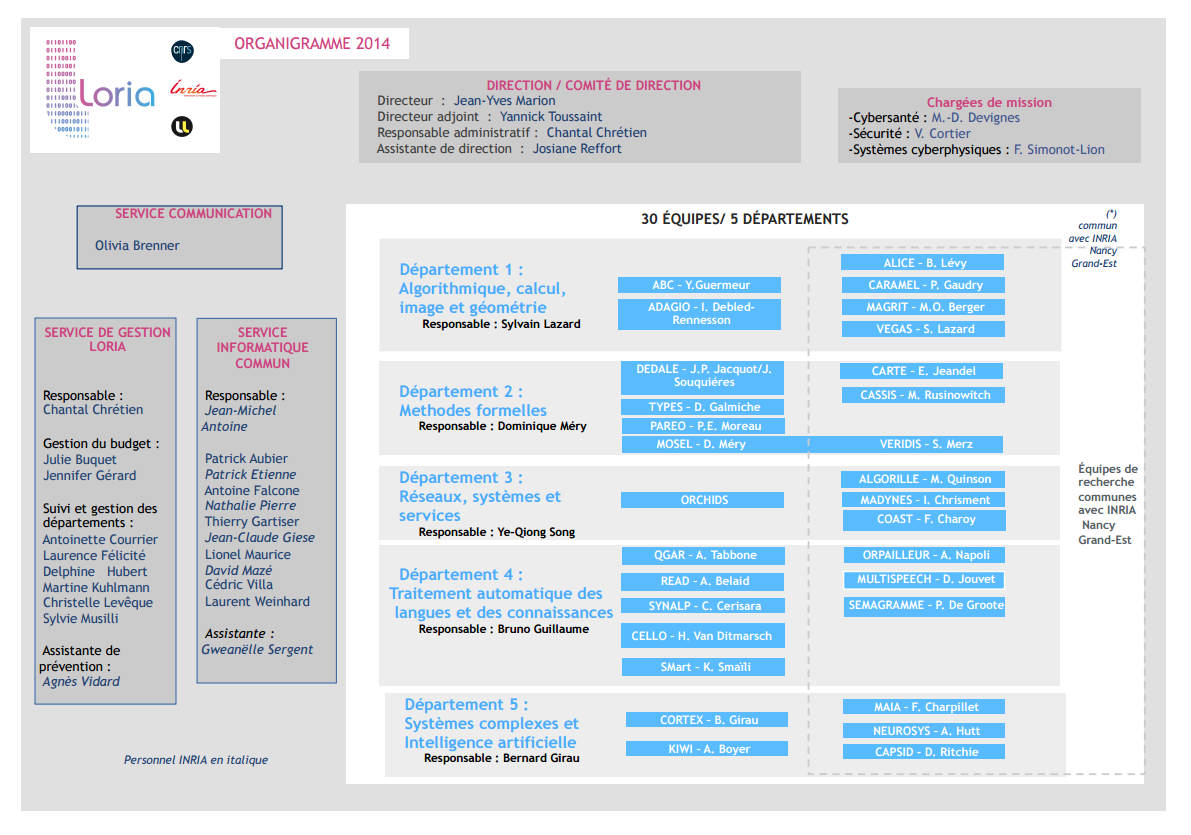
\includegraphics[width=0.9\textwidth]{figures/LORIA-organigramme}
	\caption{Organigramme du LORIA}
	\label{fig:organigramme}
\end{figure}

En tant qu'UMR, le LORIA possède sa propre administration. Un organigramme du LORIA est dispobible en \ref{fig:organigramme}, présentant la structure interne. On y remarque que même si les différentes entités administratives sont bien définies, il n'y a pas de hiérarchie directe entre elles.


\section{la "Programmer's Learning Machine"}

Le projet "Programmer's Learning Machine" (abrégé PLM) est un projet commencé en 2007 par l'équipe VERIDIS de l'INRIA.

Ce projet a pour but de fournir aux étudiants en informatique une plateforme d'initiation aux concepts de programmation basiques et avancés ainsi qu'un outil d'analyse et d'aide à la médiation pour l'enseignant.
La PLM est utilisée depuis à Telecom Nancy, et sert en première année à aider à la formation des nouveaux étudiants. Elle possède pour le moment plus de 200 exercices distincts portant sur divers sujet allant de l'introduction aux concepts de programmation à la récursivité ou aux tris.

\subsection{La PLM en tant qu'application lourde}

Dans sa forme originelle, la PLM était une application Java lourde écrite en Swing. L'utilisateur lançait le programme sur son ordinateur et obtenait des résultats. L'application lourde est aujourd'hui en version 2.6 et approche de la version 2.7.

La PLM est constituée d'exercices, regroupés en leçons et étendus sur différents univers : buggles, turmites, tortues mais aussi listes ou même simple tests sans interface particulière. Chaque exercice propose donc un scénario dans ces univers, présentant un nouveau concept à l'utilisateur.
Celui-ci doit alors trouver quel code permet de résoudre l'exercice en s'aidant de la démonstration, du texte de mission et de l'API\footnote{API : application program interface, ensemble des commandes spécifiques au programme. Ici, il s'agit des commandes de l'univers.} du monde.
\begin{figure}[h]
	\centering
		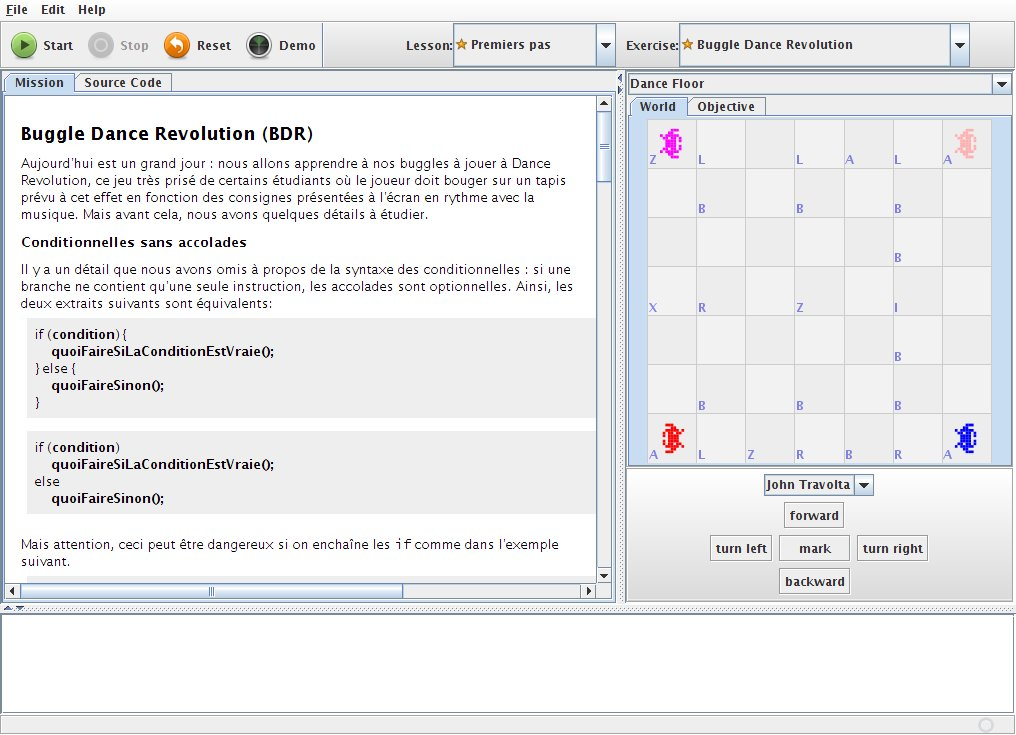
\includegraphics[width=0.9\textwidth]{figures/PLM-exercice1}
	\caption{Exemple d'exercice : Buggle Dance Revolution, portant sur la lecture d'informations et le pattern matching.}
	\label{fig:plmEx1}
\end{figure}

La PLM a été la cible de différents projets au cours du temps, de manière à ajouter des fonctionnalités : langage C, nouveaux exercices et nouvelles leçons et plus récemment aide spécifique à l'utilisateur et aux enseignants.

\subsection{Portage web de la PLM}

En plus des améliorations apportées à la PLM elle-même, il est question depuis décembre 2014 d'un portage web de l'application. Ce projet, nommé WebPLM, est principalement géré par Matthieu Nicolas.
La nouvelle architecture proposée est une interface client utilisant angular.js reliée via une WebSocket à un serveur web tournant sous Play Framework.

De cette manière, il serait en fait possible de centraliser les informations (ce qui permettrait un partage plus facile des améliorations) mais aussi pour permettre à terme de l'intégrer aux MOOC de programmation.
\begin{figure}[h]
	\centering
		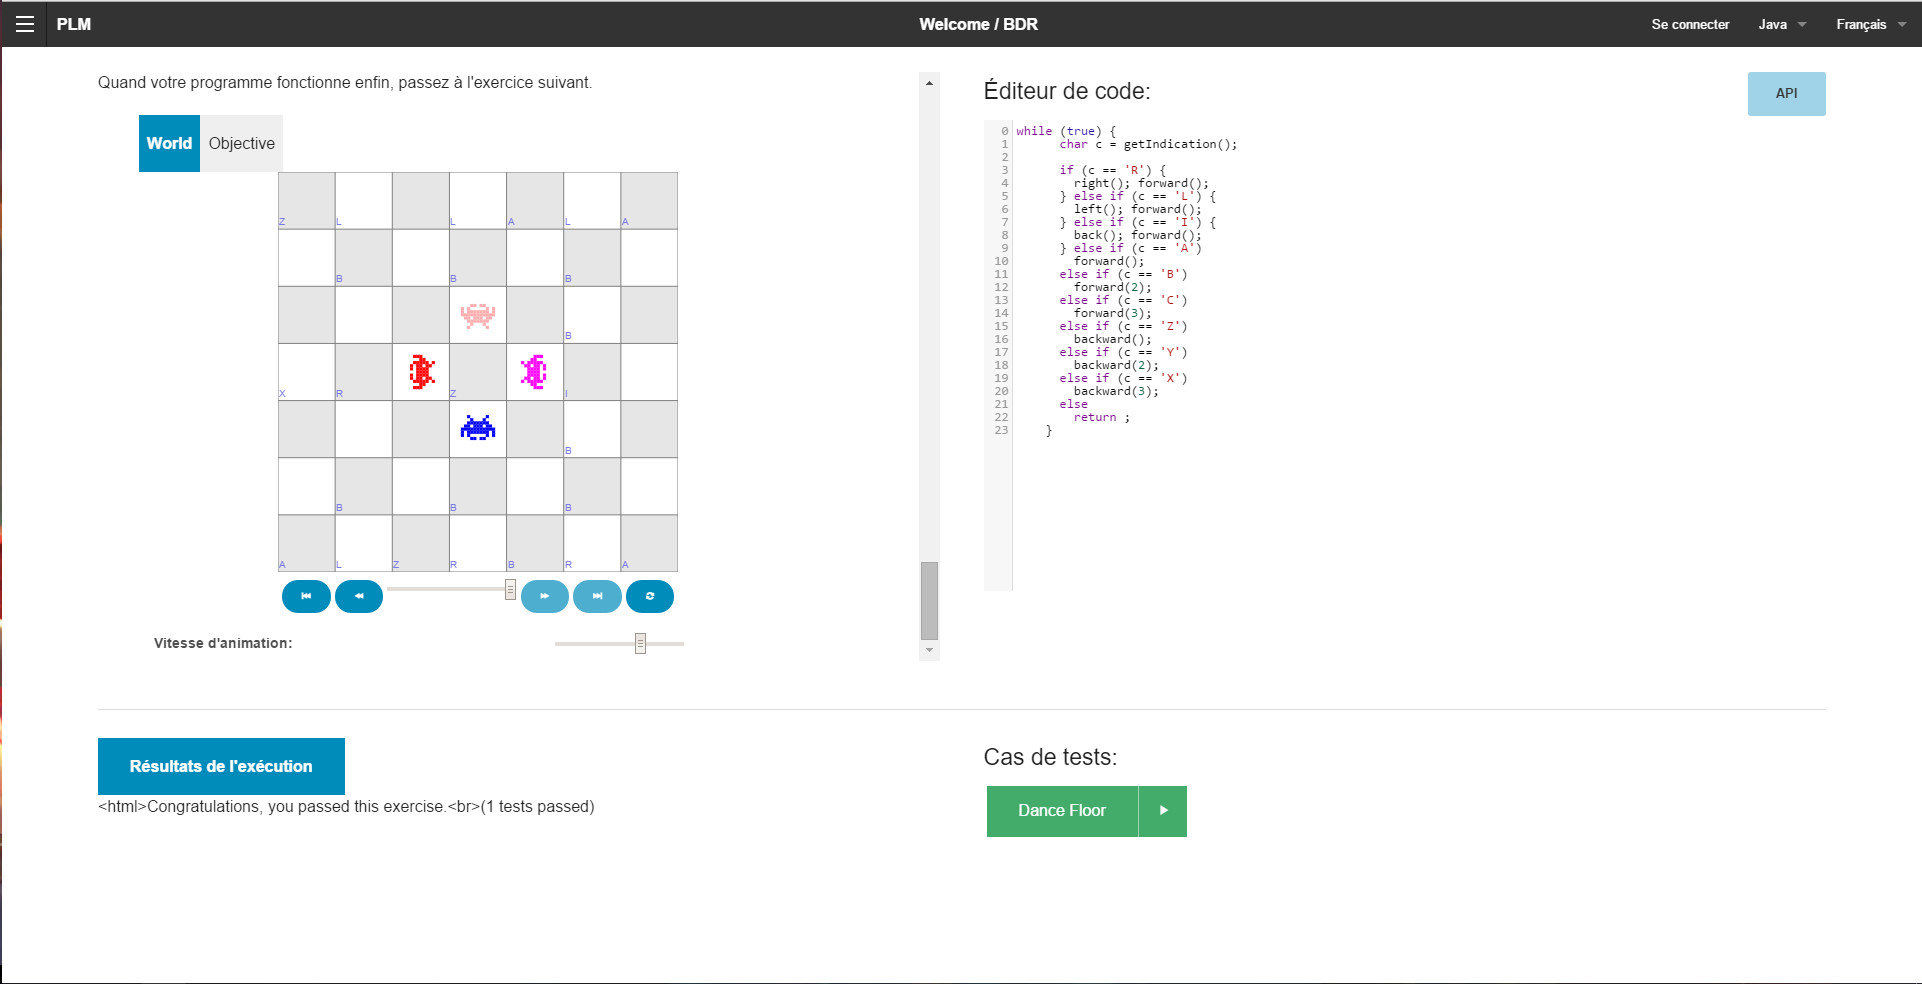
\includegraphics[width=0.9\textwidth]{figures/WebPLM-exercice1}
	\caption{Apparence de WebPLM, portage web de la PLM.}
	\label{fig:wplmEx1}
\end{figure}

Le portage web de PLM est aujourd'hui à un état utilisable, la plupart des exercices sont disponibles et les rares problèmes restants sont plus de l'ordre du confort visuel (problèmes d'affichage) ou de l'ordre de données non mises à jour.

\cleardoublepage

\chapter{Problématique du stage}

\section{Contexte du stage}

Le portage web entamé récemment portait principalement sur l'interface client et l'utilisation de PLM, sans se soucier des problèmes de performance ou de sécurité.
Le projet ayant auojurd'hui atteint un système ou son déploiement est envisageable, il est nécessaire d'adresser ces deux problèmes.

Pour pallier à cela, MM. Quinson, Oster et Nicolas ont envisagé de séparer les deux composantes principales de la PLM : l'environnement d'exécution des exercices et l'environnement d'évolution de l'élève.
Cette solution permettrait donc d'isoler l'exécution dans des environnements contrôlés et dont la performance peut être mise à l'échelle.

Cependant, la PLM n'a pas été prévue pour séparer ces deux fonctions, il fallait donc comprendre le code d'origine et mettre en place une stratégie pour le séparer.

\section{Objectifs du stage}

Ce stage avait donc pour objectif de séparer les composantes de compilation/exécution de code élève et de gestion du progrès de l'élève.

Les objectifs du stage ont donc été de :
\begin{itemize}
	\item Identifier les composantes d'exécution et de gestion de l'élève dans la PLM.
	\item Créer un outil d'exécution de code
	\item Utiliser cet outil lors de la demande d'exécution de code
	\item Rendre l'outil sécurisé et distribuable.
	\item Améliorer la PLM pour retirer les composantes inutiles
\end{itemize}

Les pistes proposées par les encadrants de stages étaient de :
\begin{itemize}
	\item Utiliser une queue de message pour stocker les informations de compilation
	\item Utiliser la technologie Docker pour rendre le système distribuable.
\end{itemize}

\cleardoublepage

\chapter{Réalisation}

\section{Environnement de réalisation}

La réalisation s'est principalement faite sur un environnement de développement Windows et un environnement d'exécution Linux.

Les technologies utilisées étaient :
\begin{description}
	\item{Docker} \hfill \\
		Docker est une technologie de gestion d'applications distribuées. Le principe est de créer des images de machines virtuelles (appelées images docker) qui, une fois lancées, sont directement utilisables avec tous logiciels lancés. \\
		Une telle technologie a pour effet de 
	\item{RabbitMQ} \hfill \\
		Rabbit MQ est un gestionnaire de queue de message. Une queue de message est un  système permettant de stocker temporairement des données par "bloc". On peut se connecter à cette queue de message pour y déposer des blocs ou en demander un. \\
		L'idée est que les clients ne s'intéressent pas à qui traite les mesages, juste à ce qu'il soit traité.
	\item{Play Framework} \hfill \\
		Play Framework est une application de déploiement de serveur web. Il permet d'installer rapidement un environnement web basé sur une JVM (java ou scala). C'est le système choisi pour développer la version web de la PLM.
\end{description}

\section{Méthode de réalisation}

\subsection{Modèle global envisagé}

\subsection{Création des juges}

\subsection{Utilisation des juges}

\subsection{Stockage du résultat}

\subsection{Analyses de performances, limites d'exécution, arrêt automatique}

\subsection{Etude d'un mode débug}

\subsection{Utilisation de Dockers}

\subsection{Agglomération des données d'opérations}

\subsection{Ajout d'opérations de logging}

\subsection{Standardisation des données}

Un problème assez particulier nous est apparu. Pour certains mondes, le code de résolution était entré et un juge avlidait le résultat, cependant l'affichage sur la WebPLM paraissait faux.

Il  s'avère que la génération de certains mondes était aléatoire, ce qui provoquait une discordance entre les actions calculées à partir du monde du juge et celles appliquées sur le monde affiché. Il a donc fallu standardiser les mondes.

Pour cela, il a été appliqué une méthode simple : les fonctions aléatoires ont vu leur "seed" se faire fixer au même nombre. Selon la Javadoc, les résultats sont donc maintenant strictement identiques.

\subsection{Documentation du code existant}

\subsection{Mise en place d'un Security Manager}

\subsection{Pré-génération des données}

\subsection{Nettoyage de la PLM}

\section{Résultats obtenus}

\subsection{Modèle final}

\cleardoublepage 

\chapter{Résultats}

\section{Bilan}

\section{Améliorations prévues}

\section {Améliorations possibles}

\cleardoublepage
\thispagestyle{empty}

\section*{Résumé}
\addcontentsline{toc}{chapter}{Résumé}

{\bf Mots-clés :}


\section*{Abstract}
\addcontentsline{toc}{chapter}{Abstract}

{\bf Keywords :}


\end{document}
